\documentclass[]{article}
\usepackage{amssymb,latexsym,amsmath}   % Standard packages
\usepackage{graphicx}
\usepackage{amsmath}
\usepackage{times}
\usepackage{color}
\usepackage{enumerate}
\usepackage{empheq}
%\usepackage{mwe}
\usepackage{subfig}
\addtolength{\textwidth}{1.1in}
\addtolength{\textheight}{1.10in}
\addtolength{\evensidemargin}{-0.75in}
\addtolength{\oddsidemargin}{-0.75in}
\addtolength{\topmargin}{-.50in}



\newcommand{\todo}[1]{ {\color{red} TODO: #1} }
\newcommand{\blue}[1]{\textcolor{blue}{#1}}
\newcommand{\red}[1]{\textcolor{red}{#1}} 


\begin{document}

\title{Modeling Inadequacy in Hierarchical Models of Supercapacitors}
\author{Danial Faghihi,
Damien Lebrun-Grandie
}
\maketitle

Development of inadequacy representations for simple zero-dimensional
models of super-capacitors was started with input from John Turner (PI) and Damien
Lebrun-Grandie at Oak Ridge. The model problem being pursued is the
up-scaling of a one-dimensional linear model that does not include
Faradaic effects. The analytic solution of this ``high fidelity'' model
is available and shows that an exact zero-dimensional non-Markovian
model can be derived in terms of a history integral. This is
impractical in general, so in this case the stochastic inadequacy
representation needs to account for the incomplete history information
available to the low-fidelity model. This suggests a formulation in
terms of an auxiliary stochastic ordinary differential equation
representing an uncertain history, and the challenge is to constrain it
to be consistent with plausible system state histories.
%---- Added by Danial
The cell voltage $V_{cell}$ for applied electrical current to the super-capacitor cell is taken into account as the quantity of interest (QoI). We used information from residual associated with solution of LF model of overpotential evolution $\eta_{LF}(\xi,\tau)$ to estimate error in QoI, $\epsilon_{QoI}=V_{cell}(\eta_{HF})-V_{cell}(\eta_{LF})$, without having to solve HF model. 
Figure (\ref{fig:cycl}) shows the spatial and temporal evolution of $\eta_{LF}$ during a cyclic charge-discharge, a common technique used to test the performance and cycle-life of energy storage devices, and the corresponding error in QoI.

%--- Danial's old paragraph
%This project aim to address model inadequacy in a set of hierarchical models for predicting behaviors of energy storage devices i.e. supercapacitors batteries. 
%Supercapacitors is a cell consists of different layers (anode collector, anode electrode, separator, cathode electrode, cathode current collector).
%The quantity of interest (QoI) in this problem is the cell voltage $V_{cell}$ for given electrical current applied to the super-capacitor cell. We consider hierarchical models, with different fidelities and computational costs, for the spatial and temporal evolution of overpotential $\eta$ in electrodes:  
%high-fidelity (HF) model;
%using simplified assumptions regarding the material and responses to build an intermediate-fidelity (IF) model; and through averaging to construct the low-fidelity (LF) model.
%We have access to finite element code for solution of the HF model, \textit{cap}, through collaboration with John Turner (PI) in Oak Ridge National Laboratory.
%We aim to address modeling error due to the upscaling the models. Particularly, we use information from residual associated with solution of LF model $\eta_{LF}$ to estimate error in QoI, $\epsilon_{QoI}=V_{cell}(\eta_{HF})-V_{cell}(\eta_{LF})$, without having to solve HF model. 
%Figure (\ref{fig:cycl}) shows the spatial and temporal evolution of $\eta_{LF}$ during a cyclic charge-discharge, a common technique used to test the performance and cycle-life of energy storage devices, and the corresponding error in QoI.

\begin{figure}[h]
    \centering
    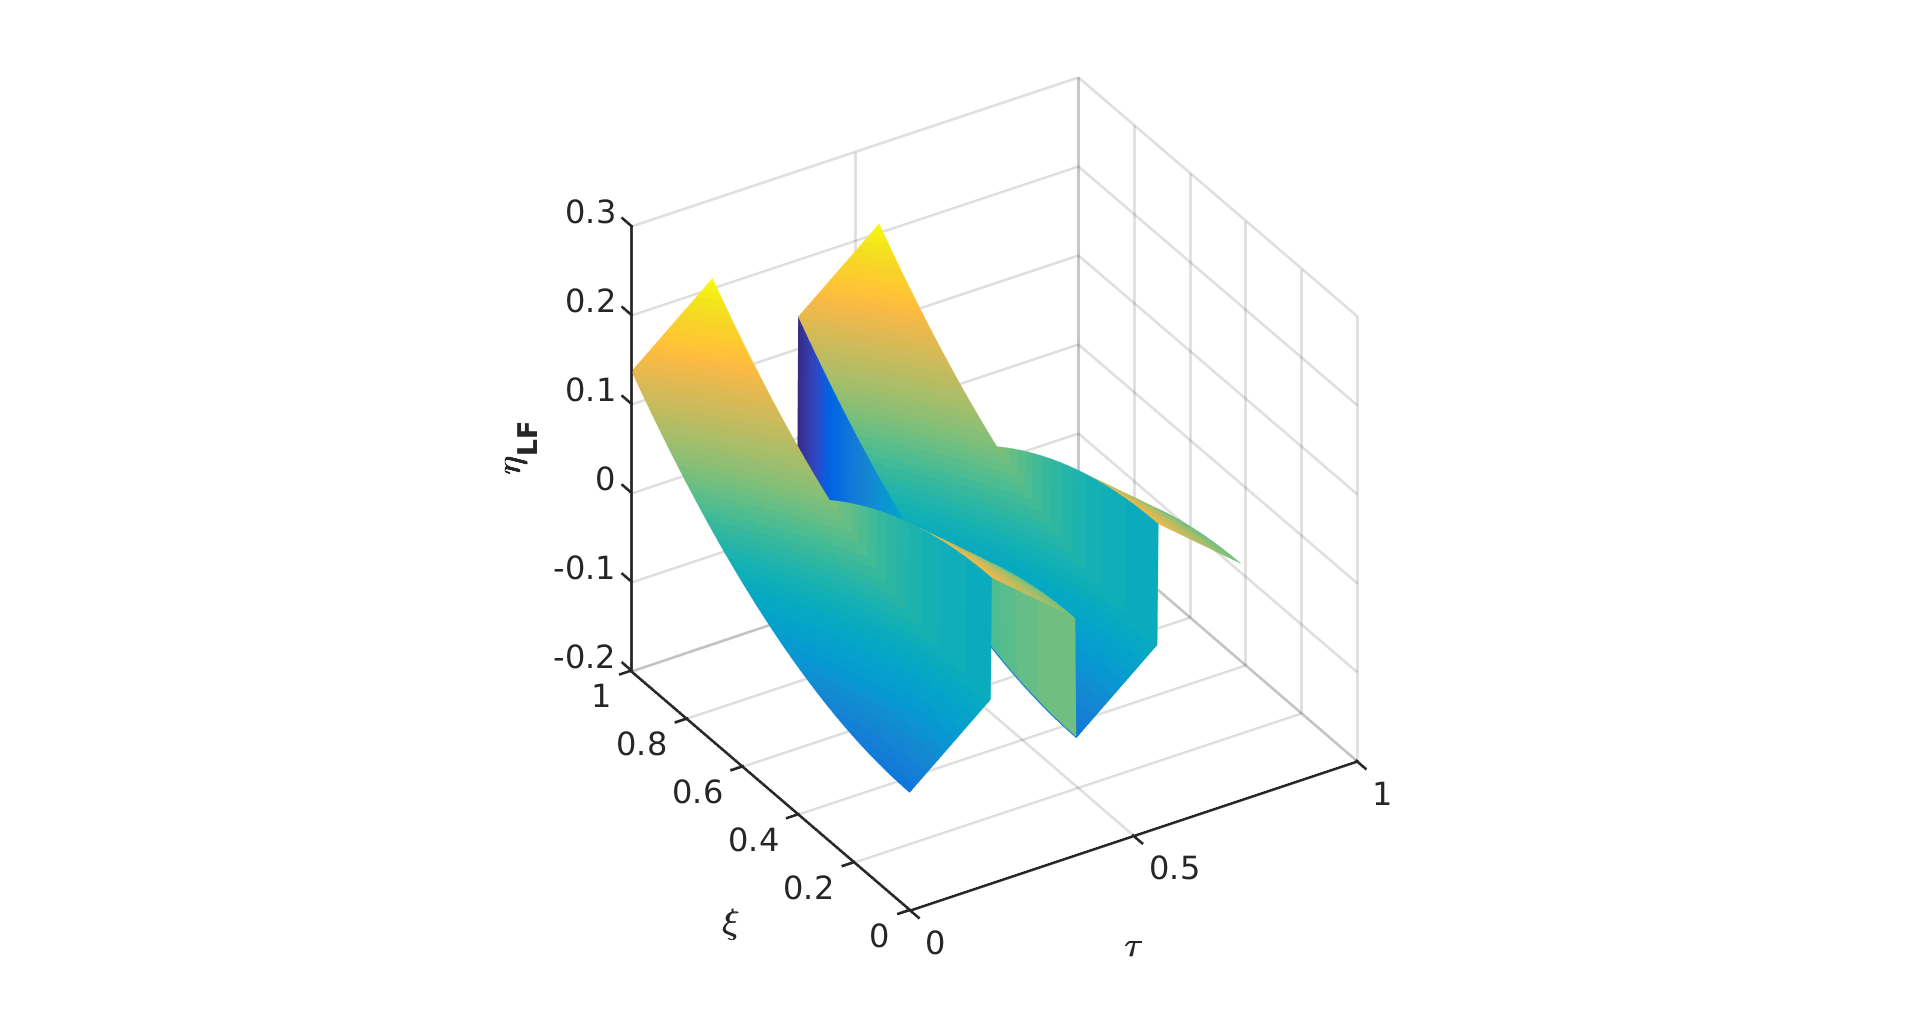
\includegraphics[trim = 5in 0in 5in 0in, clip, width=0.45\textwidth]{etaLF.png}
    ~
    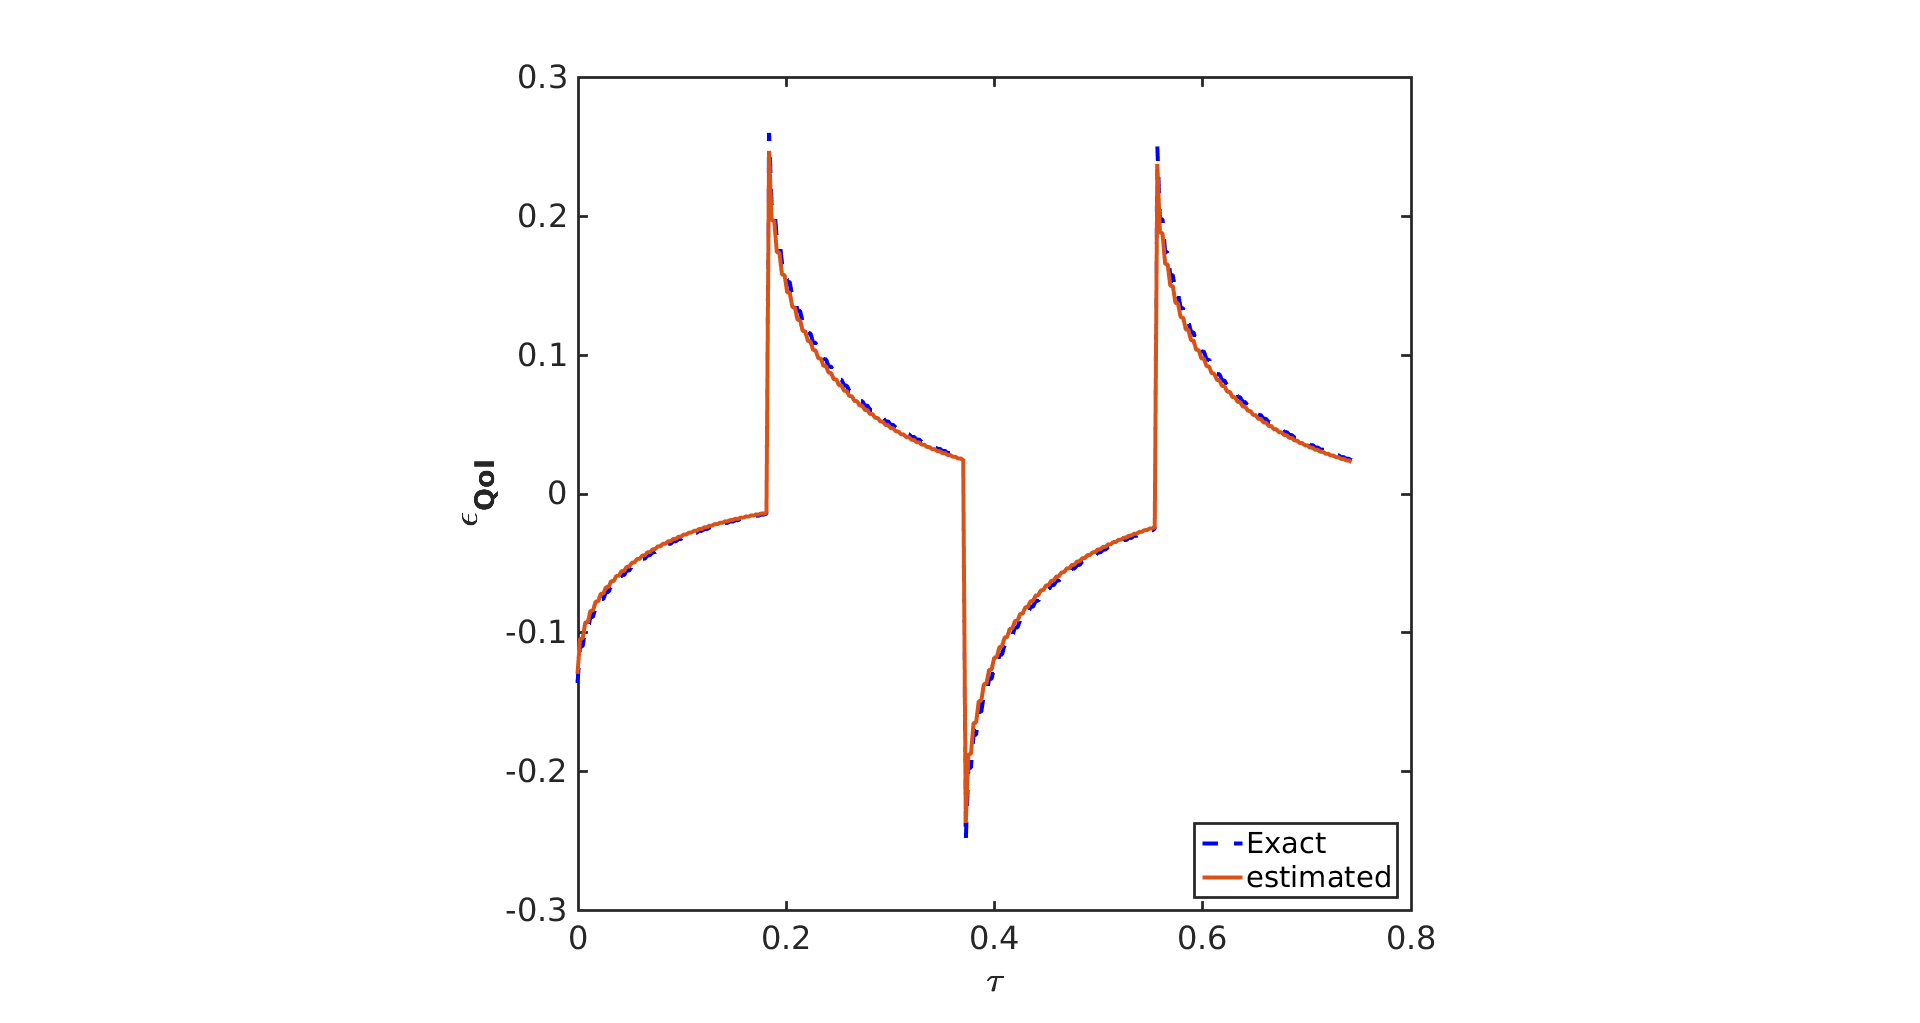
\includegraphics[trim = 4in 0in 4in 0in, clip, width=0.45\textwidth]{E_qoi.png}       
    \caption{(left) Solution of LF model $\eta$ at different normalized time $\tau$ and space $\xi$; (right) comparison of the estimated and exact error in QoI using LF and IF models $\epsilon_{QoI}=V_{cell}(\eta_{HF})-V_{cell}(\eta_{IF})$.}
    \label{fig:cycl}
\end{figure}



\end{document}
